\chapter{Introduction}
Game theory is a set of analytical tools and solution concepts, which provide
explanatory and predicting power in interactive decision situations, when the
aims, goals and preferences of the participating players are potentially in
conflict, Szabo and Fath (2007) \cite{Szabo2007}. The Prisoner's Dilemma(PD) is a well
known example in Game Theory and in recent years has become the gold standard of
understanding evolution of co-operative behavior \cite{Lorberbaum1994}.
Thus, it has been a topic of focus in various fields, such as biology,
sociology, ecology and psychology.

In the example of the Prisoner's Dilemma(PD) two criminals have been arrested
and interrogated, with no way of communicating, by the police. They are given
only two choices, to either cooperate with each other or to defect.
Consider that the prisoners would be put back in their cells and would be asked
the same question tomorrow. Furthermore, let this happen repeatably. This is
referred to as the Iterated Prisoner's Dilemma(IPD) an example that has been a
rich source of research material since the 1950s but has earned much interest in
the 1980s due to the work done by the political scientist Robert Axelrod
\cite{Axelrod1980a, Axelrod1980b, Axelrod1981}.

In 1980, Axelrod held the first ever IPD computer tournaments \cite{Axelrod1980a,
Axelrod1980b}, he invited
academia from various fields to submit their strategies in computer code. The
tournaments were of a round robin topology, the first competition included thirteen
strategies, while the second one sixty-four. In both tournaments the strategy Tit
for Tat was announced the winner and for many years it was considered to be the
most successful strategy. Tit for Tat is a deterministic strategy that will
always cooperate in the first round and afterwards it copies the opponents last
move.

A large volume of literature emerged on the topic following this, including some
criticism about these initial tournaments. Scientists questioned whether the
conditions that the first tournament took place favored Tit for Tat~\cite{RePEc:mtp:titles:0262023636}.
An argument was that the initial tournaments though they included
a 1\% chance of players misunderstanding their opponent's move in any round
,they did not examine noise. Noise is the probability
that the player will submit the wrong move. David and Vivian Kraines \cite{kraines-1989a}
stated that, Tit for Tat performed rather poorly when noise was introduced in the tournament.
Another aspect, is the payoff matrix, which according to Kretz \cite{Kretz2011},
effects the results.

Furthermore, another aspect needed to be taken into account is the network
topology underlying the tournament. In 1992 Nowak's and May's paper \cite{Nowak1992},
spatial tournament are introduced. In which the players are placed on an two-
dimensional spatial array and allowed to play a game with only the immediate neighbors.
Thus, squares that are adjoint. An example of this is shown in Figure~\ref{fig:nowak-example}.

\begin{figure}[!hbtp]
	\centering
		\begin{tikzpicture}

\matrix (input) [matrix of nodes,
                nodes={rectangle, draw=black, minimum size=1cm}] at (0,0)
{
|[fill=white!20]| & |[fill=white]|     & |[fill=white]|      &    |[fill=white]|     &    |[fill=white]|    \\
|[fill=white]| & |[fill=white]|     & |[fill=black!20]|   &    |[fill=white]|     &    |[fill=white]|    \\
|[fill=white]| & |[fill=black!20]|  & |[fill=black]|      &    |[fill=black!20]|  &    |[fill=white]|    \\
|[fill=white]| & |[fill=white]|     & |[fill=black!20]|      &    |[fill=white]|     &    |[fill=white]|    \\
|[fill=white]| & |[fill=white]|     & |[fill=white]|      &    |[fill=white]|     &    |[fill=white]|    \\
};
%\node [draw] at (input.south) {};

\end{tikzpicture}

		\caption{Topology of Nowak's Tournament}
  \label{fig:nowak-example}
\end{figure}

Their tournament considered the PD and the players could only defect or
cooperate.  They provided proof that cooperative behavior can emerge from a PD
tournament in spatial topology. Many works on the IPD and spatial tournament
were held due to their original paper. Such as \cite{Grujic2014, Nowak1993,
Maciver1992, Nowak1992, Brauchli1999, Meng2015, Lindgren1994}.
These tournaments use either the PD or IPD and simple to complex strategies.

One can argue that the real life interactions are better represented by spatial
tournament because in real life not all players interact with all opponents.
Additionally, an interesting aspect of the spatial topology are the results
compared to those of a round robin tournament. This dissertation will be focusing on
reproducing a spatial tournament with some of the most successful strategies of
various tournaments that have been held.

For replicating the spatial topology, various graphs have been used, compared to
other woks which have used only lattices. Graphs such as, cyclic,
small world, random and complete. The affects of the topology on the
effectiveness of these strategies, has been studied. Followed by the attempt to
use a genetic algorithm to train a strategy that performs well in any given
topology.

\section{The Prisoner's Dilemma}
The PD was originally formulated in Merril \cite{Flood1958},
who were working on the Flood-Desher Experiment at the RAND cooperation in 1950.
Later in 1950, the mathematician Albert W. Tucker presented the first formal
representation of the PD, titled  A Two-Person Dilemma in a seminar at
Stanford University \cite{GassAssad2005}.

A description of the PD, found in \cite{Li2011} is as follows:
There are two players that simultaneously have to decide to whether Cooperate (C)
or Defect (D) with each other, without exchanging information.

\begin{itemize}
  \item If both players choose to cooperate they will both receive a reward (R)
  \item If a player defects and the other cooperates then the defector receives
  a temptation payoff (T) and the cooperator a sucker payoff (S)
  \item If both players defect they will both receive a penalty (P)
\end{itemize}

Figure~\ref{fig:pd_payoff} illustrates the payoffs matrix.

\begin{figure}[h!]
    \centering
    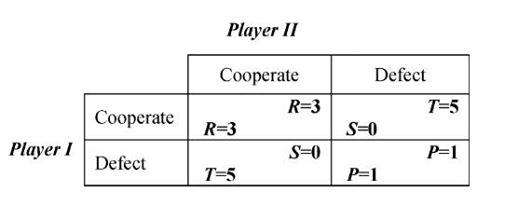
\includegraphics[scale=0.45]{chapter-one/pd_payoff.jpg}
    \caption{The payoff matrix for the Prisoners Dilemma}
    \label{fig:pd_payoff}
\end{figure}

Taking into account the assumptions that both players are rational
and that there is no way of communication between them. No matter what the
other player does, defecting will be their dominant choice as it yields a higher
payoff than cooperation.
Thus a pure Nash Equilibrium exists when both players defect. Even though, both
players would do better if they were to cooperate.Thus creating the dilemma.

Furthermore, for this to hold there are some extra assumptions for the
relationship of the four outcomes. The T temptation to defect has to offer the
highest payoff for a player and the worst he could get has to be the sucker S.
Likewise, the reward for mutual cooperation should exceed that of mutual
defection P. Thus the next condition is~\ref{firstassum}:

\begin{equation}\label{firstassum}
 T > R > P > S
\end{equation}

Moreover, it is assumed that the average of T and S is less than the reward for
mutual cooperation~\ref{secondassum} :

\begin{equation}\label{secondassum}
    R > (T+S)/2
\end{equation}

Same conditions such as rationality, no communication and (~\ref{firstassum}),
(~\ref{secondassum}),
apply for the IPD. An IPD is nothing more than a PD were
the players interact for an infinite number of times.

\section{Problem Description}
Axelrod's tournaments set a seed for generations of tournaments in the
Prisoner's using computer modeling. Research has shown that by altering the
environment of a tournament the effectiveness of some strategies can change
radically. An aspect that has been investigated as to how the tournament results
can bee affected was the topology. Nowak and May \cite{Nowak1992} introduced the spatial topology
only to set yet another seed in the PD tournaments. Even so, spatial topology
still has not been fully explored with only a small number of papers focusing on
this specific topology.  A goal of this dissertation is to understand the
current state of the art in spatial prisoner’s dilemma tournaments.

As described in \cite{MacLane1971} the contemporary world is full of networks. That
is one of the main reasons this dissertation will be focusing on such topology.
Work done at this point consider spatial topology to be that of a square lattice
were each edge represents a player which interacting/playing with only his
neighbors in their von Neuman or Moore's neighborhood. A von Neuman neighborhood
comprises the four cells orthogonally surrounding a central cell where the
Moore's neighborhood eight cells. As shown in Figure~\ref{fig:neighborhood}.

\begin{figure}[!hbtp]
	\centering
	\begin{subfigure}[h]{0.45\textwidth}
		\centering
		\begin{tikzpicture}

	\matrix (input) [matrix of nodes,
	nodes={rectangle, draw=black, minimum size=1cm}] at (0,0)
	{
		|[fill=white!20]| & |[fill=white]|        & |[fill=white]|      &    |[fill=white]|     &    |[fill=white]|    \\
		|[fill=white]|    & |[fill=white!20]|     & |[fill=red!20]|     &    |[fill=white]|     &    |[fill=white]|    \\
		|[fill=white]|    & |[fill=red!20]|       & |[fill=red]|        &    |[fill=red!20]|    &    |[fill=white]|    \\
		|[fill=white]|    & |[fill=white!20]|     & |[fill=red!20]|     &    |[fill=white]|     &    |[fill=white]|    \\
		|[fill=white]|    & |[fill=white]|        & |[fill=white]|      &    |[fill=white]|     &    |[fill=white]|    \\
	};
	%\node [draw] at (input.south) {};

\end{tikzpicture}

		\caption{von Neuman's neighborhood}
	\end{subfigure}
	\hfill
	\begin{subfigure}[h]{0.52\textwidth}\centering
		\centering
		\begin{tikzpicture}

	\matrix (input) [matrix of nodes,
	nodes={rectangle, draw=black, minimum size=1cm}] at (0,0)
	{
		|[fill=white!20]| & |[fill=white]|      & |[fill=white]|      &    |[fill=white]|      &    |[fill=white]|    \\
		|[fill=white]|    & |[fill=red!20]|     & |[fill=red!20]|     &    |[fill=red!20]|     &    |[fill=white]|    \\
		|[fill=white]|    & |[fill=red!20]|     & |[fill=red]|        &    |[fill=red!20]|     &    |[fill=white]|    \\
		|[fill=white]|    & |[fill=red!20]|     & |[fill=red!20]|     &    |[fill=red!20]|     &    |[fill=white]|    \\
		|[fill=white]|    & |[fill=white]|      & |[fill=white]|      &    |[fill=white]|      &    |[fill=white]|    \\
	};
	%\node [draw] at (input.south) {};

\end{tikzpicture}

		\caption{Moore's neighborhood}
	\end{subfigure}
  \caption{Possible neighborhoods. (a) A von Neuman's networ where each node has four neighbors.
  (b) A Moore's network where each node has eight neighbors}
  \label{fig:neighborhood}
\end{figure}

Some further work address the spatial topology in a variate of graphs
\cite{Dresher1992a, Szabo2007, Lutz2013, Meng2015}.
This dissertation will also follow this approach. Szabo and Fath dealt with
numerous graphs such as, lattices, small- world, scale free graphs and evolving
networks. Here a spatial topology is considered any given network where the
players are the nodes and only play other nodes that are linked to by
an edge.

Another disadvantage of the aforementioned work is that it lacked in terms of
best practice of reproducibility \cite{Axelrod1980a,Axelrod1980b,Stephens2002,Chong2004,Stewart2013}.
Due the work done by the Axelrod library \cite{axelrodproject}.
An open source python package which allows for the easy
reproducibility of experiments. As it allow to reproduce an IPD tournament and
chose between 132 strategies already given by the library. Code written for the
purpose of this dissertation has been contributed to the library: see
\url{https://github.com/Axelrod-Python}.

\section{Analysis Tools}
Due to the high computational cost of the analysis considered, Cardiff
University's super computer, Raven, is used~\cite{raven}. All the scripts and pbs
file, for producing data with Raven can be found on can be found on github:
\url{https://github.com/Nikoleta-v3/jobs}.Furthermore, all data produced for
this work is archived using zenodo and can be readily downloaded. Details are
available in Appendix~\ref{appendix}.

For the data analysis the following libraries have been used:

\begin{multicols}{2}
	\begin{itemize}
		\item Numpy 1.11.1~\cite{numpy}
		\item Pandas 0.18.1~\cite{pandas}
		\item Matplotlib 1.5.1~\cite{matplot}
		\item Scipy: 0.18.0~\cite{scipy}
		\item Networkx 1.11~\cite{networkx}
    \item Scikit learn 0.17.1~\cite{scikit}
	\end{itemize}
\end{multicols}

\section{Structure of Dissertation}
This dissertation is organized into 6 Chapters. Following this introduction:
\begin{itemize}
  \item In~\autoref{chap:Two}, as well as introducing basic graph theory, all
        previous literature dedicated to the PD/IPD and tournaments that have
        been conducted, different topologies and evolution, have been reviewed
  \item In~\autoref{chap:Three} the main software contribution of this thesis is
        described: adding topologies to the Axelrod-Python software package.
        Some initial experiments and investigations are also carried out
  \item In~\autoref{chap:Four} a more in depth analysis in the topologies affects
				and the strategies performance is studied, by using various complex
				networks as the spatial tournaments topology
  \item In~\autoref{chap:Five} using a sophisticated evolutionary algorithm a
				new strategy is trained following the work conducted by Professor M Jones
				for his currently wining strategy EvolvedLookerUp
  \item In~\autoref{chap:Six} the results of this dissertation, as well as some
				further ideas for research are presented
\end{itemize}
